\section{Results}
\label{hptpcPaper:sec:Results}

	\begin{figure}[ht]
		\begin{minipage}[t]{0.48\textwidth}
			\centering
			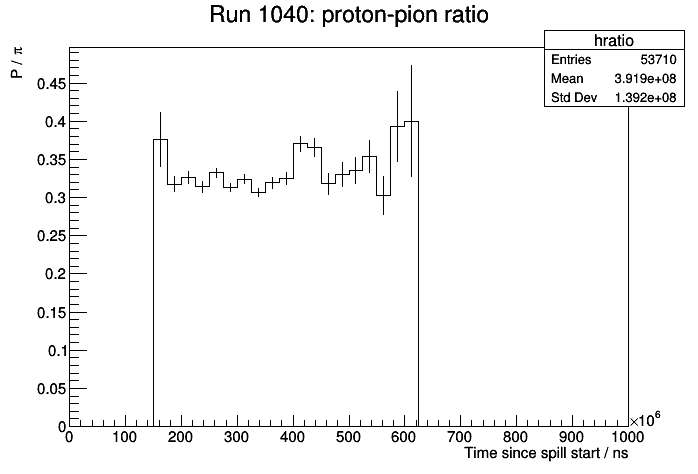
\includegraphics[width=\textwidth]{files/Figures/Run1040_proPiRatio}
			\caption{The ratio of protons to pions as a function of time since the start of the beam spill. For these data, 1 moderator block was in place and the beam momentum was nominally 0.8~GeV/c. The data for this graph is from the sum of 255 spills.}
			\label{fig:proPiRatio}
		\end{minipage} 
		\hspace{0.3cm}
		\begin{minipage}[t]{0.48\textwidth}
			\centering
			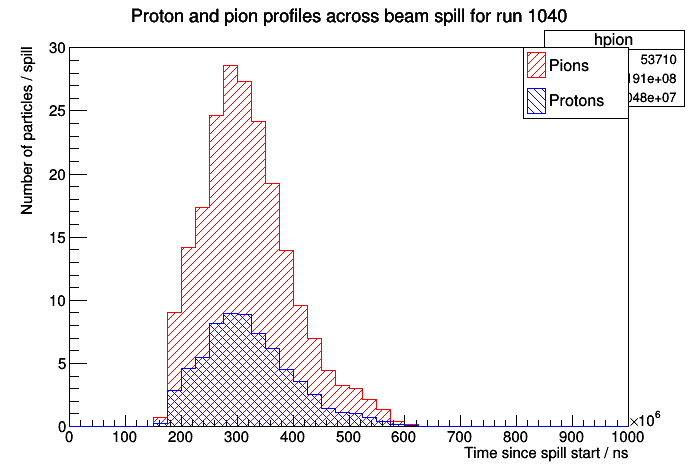
\includegraphics[width=\textwidth]{files/Figures/Run1040_proPiProf}
			\caption{The number of protons and pions detected per spill by the DsToF as a function of time since the start of the beam spill. For these data, 1 moderator block was in place and the beam momentum was nominally 0.8~GeV/c. The data for this graph is from the sum of 255 spills.}
			\label{fig:proPiProf}
		\end{minipage}
	\end{figure}

	Figure~\ref{fig:dtof_nmodblocks} shows the variation in the time of flight spectrum as recorded by the DsToF with a changing number of moderator blocks. The configuration used for most of the run was with 4 moderator blocks. 
			
	

   	\begin{figure}[h]
        \centering
	    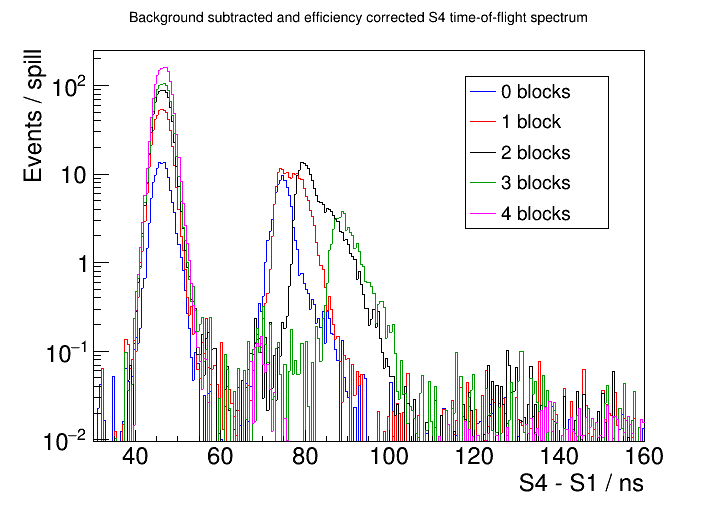
\includegraphics[width=0.7\linewidth]{files/Figures/s4ToF_axisAdj.png}
        \caption{$S_{4}$ time-of-flight spectra for varying numbers of moderator blocks. For all configurations, an exponentially falling background has been fitted and subtracted from the data. Additionally, the plot has also been corrected for the differing efficiencies of the various bars.}
        \label{fig:dtof_nmodblocks}	
   	\end{figure}
   
   	\begin{figure}[ht]
   		\begin{minipage}[t]{0.48\textwidth}
   			\centering
	   		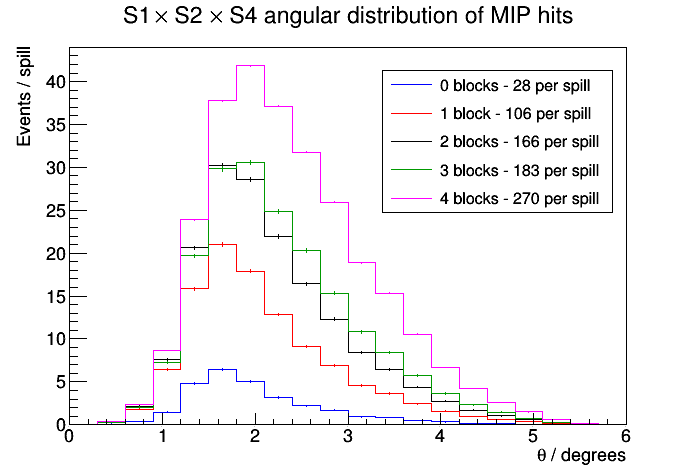
\includegraphics[width=\textwidth]{files/Figures/piS4Horz}
	   		\caption{Distribution of hits identified in $S_{4}$ as minimum ionizing particles as a function of the number of moderator blocks and the horizontal off-axis angle, as measured from $S_{1}$.}
   		\end{minipage}
   		\hspace{0.3cm}
   		\begin{minipage}[t]{0.48\textwidth}
   			\centering
   			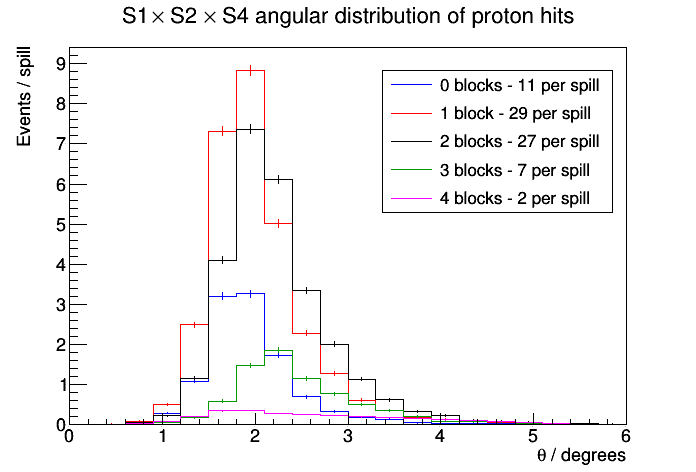
\includegraphics[width=\textwidth]{files/Figures/proS4Horz}
   			\caption{Distribution of hits identified in $S_{4}$ as protons as a function of the number of moderator blocks and the horizontal off-axis angle, as measured from $S_{1}$.}
   		\end{minipage} \\
   	
   		\begin{minipage}[t]{0.48\textwidth}
   			\centering
   			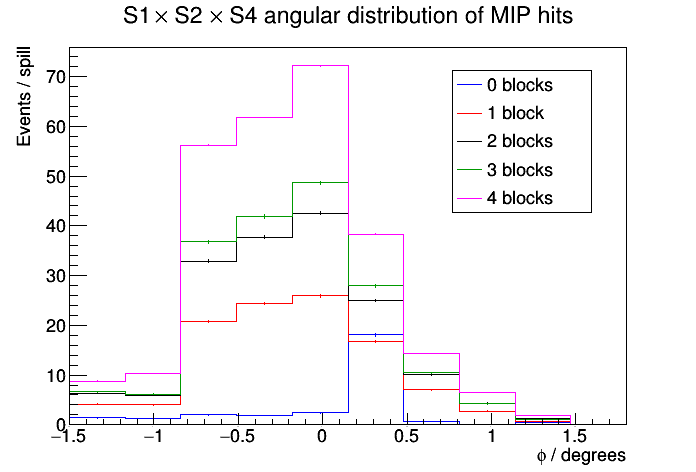
\includegraphics[width=\textwidth]{files/Figures/piS4Vert}
   			\caption{Distribution of hits identified in $S_{4}$ as minimum ionizing particles as a function of the number of moderator blocks and the vertical off-axis angle, as measured from $S_{1}$.}
   		\end{minipage}
   		\hspace{0.3cm}
   		\begin{minipage}[t]{0.48\textwidth}
   			\centering
   			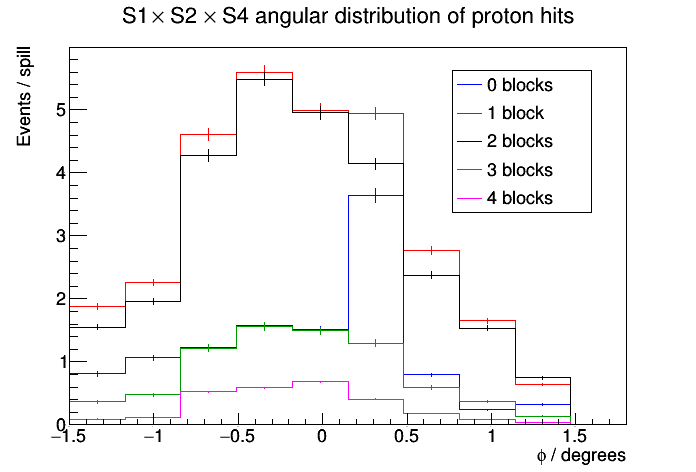
\includegraphics[width=\textwidth]{files/Figures/proS4Vert}
   			\caption{Distribution of hits identified in $S_{4}$ as protons as a function of the number of moderator blocks and the vertical off-axis angle, as measured from $S_{1}$.}
   		\end{minipage}
   	
	\end{figure}	
        
   	\begin{figure}[ht]
   		\begin{minipage}[t]{0.48\textwidth}
   			\centering
   			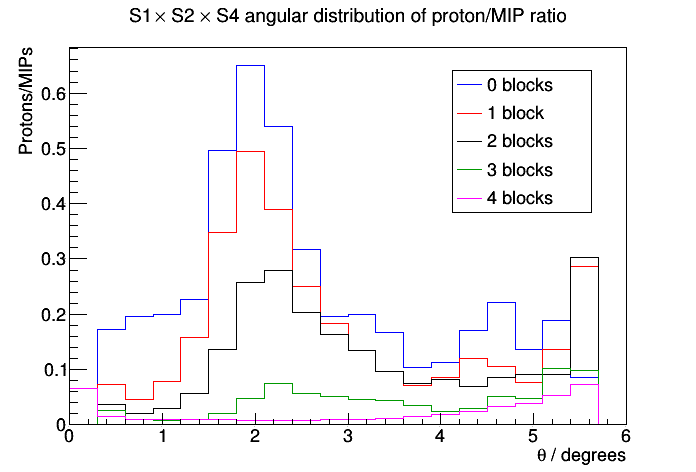
\includegraphics[width=\textwidth]{files/Figures/ratioS4Horz}
   			\caption{Proton/MIP ratio in $S_{4}$ for varying numbers of moderator blocks as a function of horizontal off-axis angle, as measured from $S_{1}$}
   			\label{fig:propiratio_s4_horz}
   		\end{minipage}
   		\hspace{0.3cm}
    	\begin{minipage}[t]{0.48\textwidth}
    		\centering
    		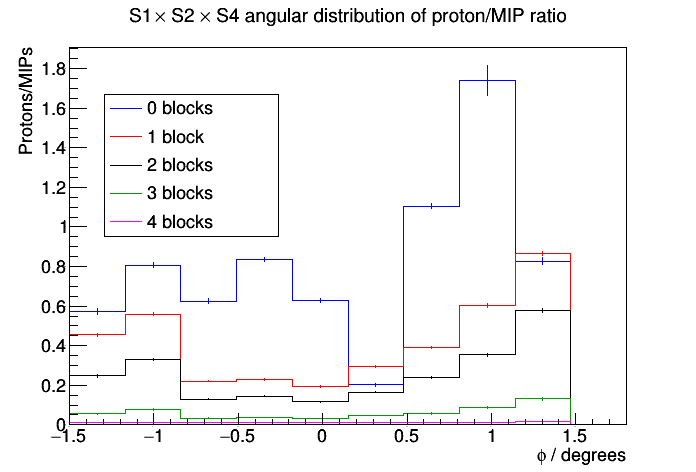
\includegraphics[width=\textwidth]{files/Figures/ratioS4Vert}
    		\caption{Proton/MIP ratio in $S_{4}$ for varying numbers of moderator blocks as a function of vertical off-axis angle, as measured from $S_{1}$}
    		\label{fig:propiratio_s4_vert}
    	\end{minipage}	
   	\end{figure}
   
	

Exact UToF and DToF figures TBD